\subsection{Stratified annotation coverage}
The September 21 export replaces the earlier Gemma error-weighted sample and GPT-OSS corpus-prefix labels. Each model has 100,000 selected sentences, drawn with seed 42 from one completion per source problem, with quotas proportional to dataset $\times$ correctness $\times$ reasoning-length-quartile supply. The four 25,000-sentence parts are merged, not independent experimental replicates. GPT-OSS uses the corrected length-based sampling plan, which falls back to replay tokens when server reasoning-token counts are zero.
GPT-OSS contributes 100,000 valid labels on 1,510 problems; Gemma contributes 99,999 on 1,503 problems. One Gemma sentence has a missing judge response and is excluded; its trace remains partially labelled. Both models now have class-token coverage on all six benchmarks. Sampled class populations remain smaller than the full 4,647-attempt corpus and need not contain the same problems across models. Sampling eligibility uses the saved scored-trace population; subsequently retained invalid answers in the full-corpus accuracy analysis do not imply annotation eligibility.
\begingroup\scriptsize\setlength{\tabcolsep}{4pt}
\begin{longtable}{@{}llrrr@{}}
\caption{Stratified annotation population. Problems each contribute one labelled completion; valid labels are sentence counts, not token counts. Missing labels are retained in the sampling record.}\label{tab:stratified-labels}\\
\toprule
Model & Dataset & Problems & Valid labels & Missing \\
\midrule\endfirsthead
\multicolumn{5}{l}{\textit{Continued from previous page}}\\
\toprule
Model & Dataset & Problems & Valid labels & Missing \\
\midrule\endhead
\bottomrule\endfoot
Gemma & MATH-500 & 494 & 20,825 & 0 \\
Gemma & AIME24 & 30 & 2,887 & 0 \\
Gemma & AIME25 & 30 & 3,861 & 0 \\
Gemma & Olympiad & 639 & 54,556 & 1 \\
Gemma & AMC23 & 40 & 2,573 & 0 \\
Gemma & Minerva & 270 & 15,297 & 0 \\
GPT-OSS & MATH-500 & 496 & 14,050 & 0 \\
GPT-OSS & AIME24 & 30 & 4,128 & 0 \\
GPT-OSS & AIME25 & 30 & 4,987 & 0 \\
GPT-OSS & Olympiad & 642 & 70,215 & 0 \\
GPT-OSS & AMC23 & 40 & 1,373 & 0 \\
GPT-OSS & Minerva & 272 & 5,247 & 0 \\
\end{longtable}\endgroup

\begin{figure}[p]\centering
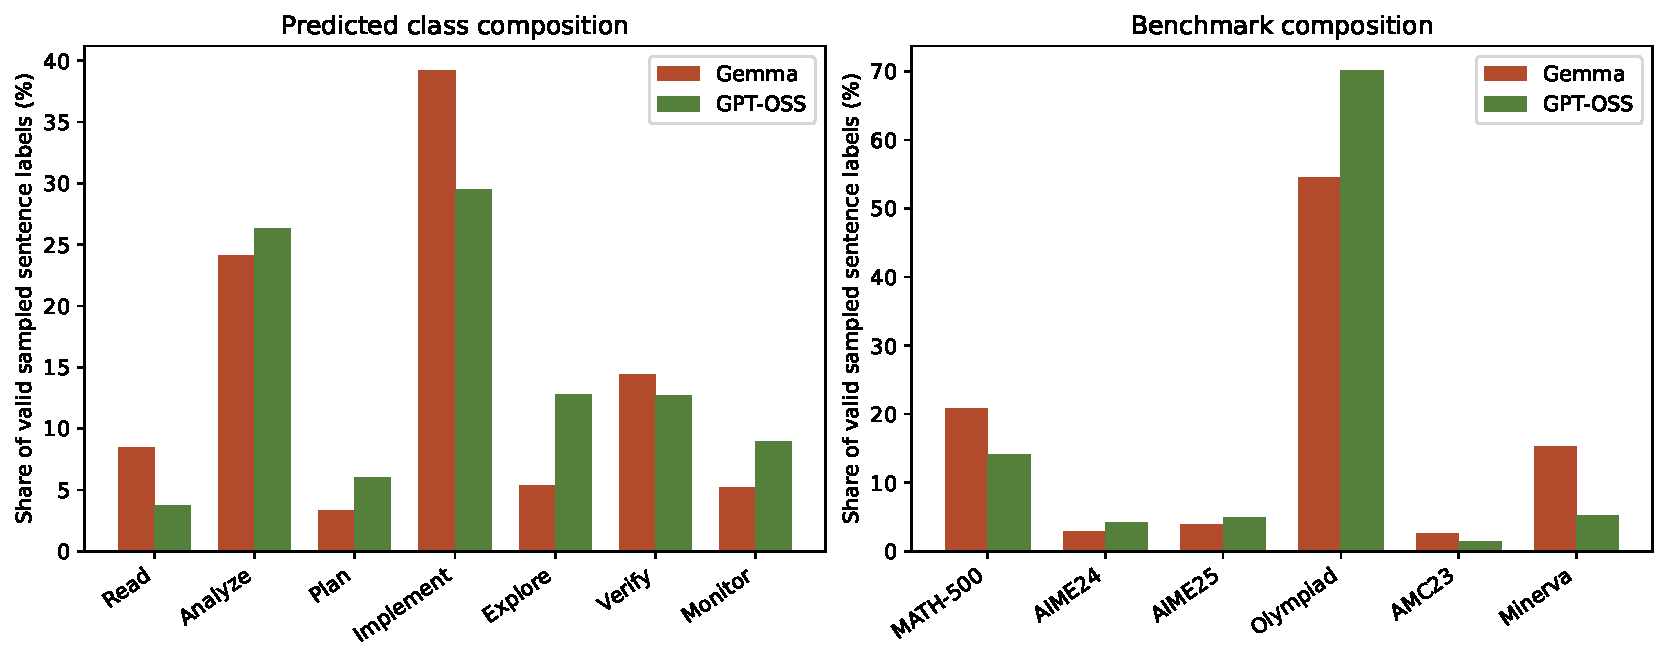
\includegraphics[width=\linewidth]{figures/stratified_label_composition.pdf}
\caption{Gemma and GPT-OSS stratified label composition. Denominators are 99,999 and 100,000 valid sampled sentences. Equal sample budgets do not imply equal class or benchmark proportions. These sentence shares are neither complete-corpus token shares nor adjusted model effects.}
\Description{Gemma and GPT-OSS stratified label composition. Denominators are 99,999 and 100,000 valid sampled sentences. Equal sample budgets do not imply equal class or benchmark proportions. These sentence shares are neither complete-corpus token shares nor adjusted model effects.}
\end{figure}

\begin{figure}[p]\centering
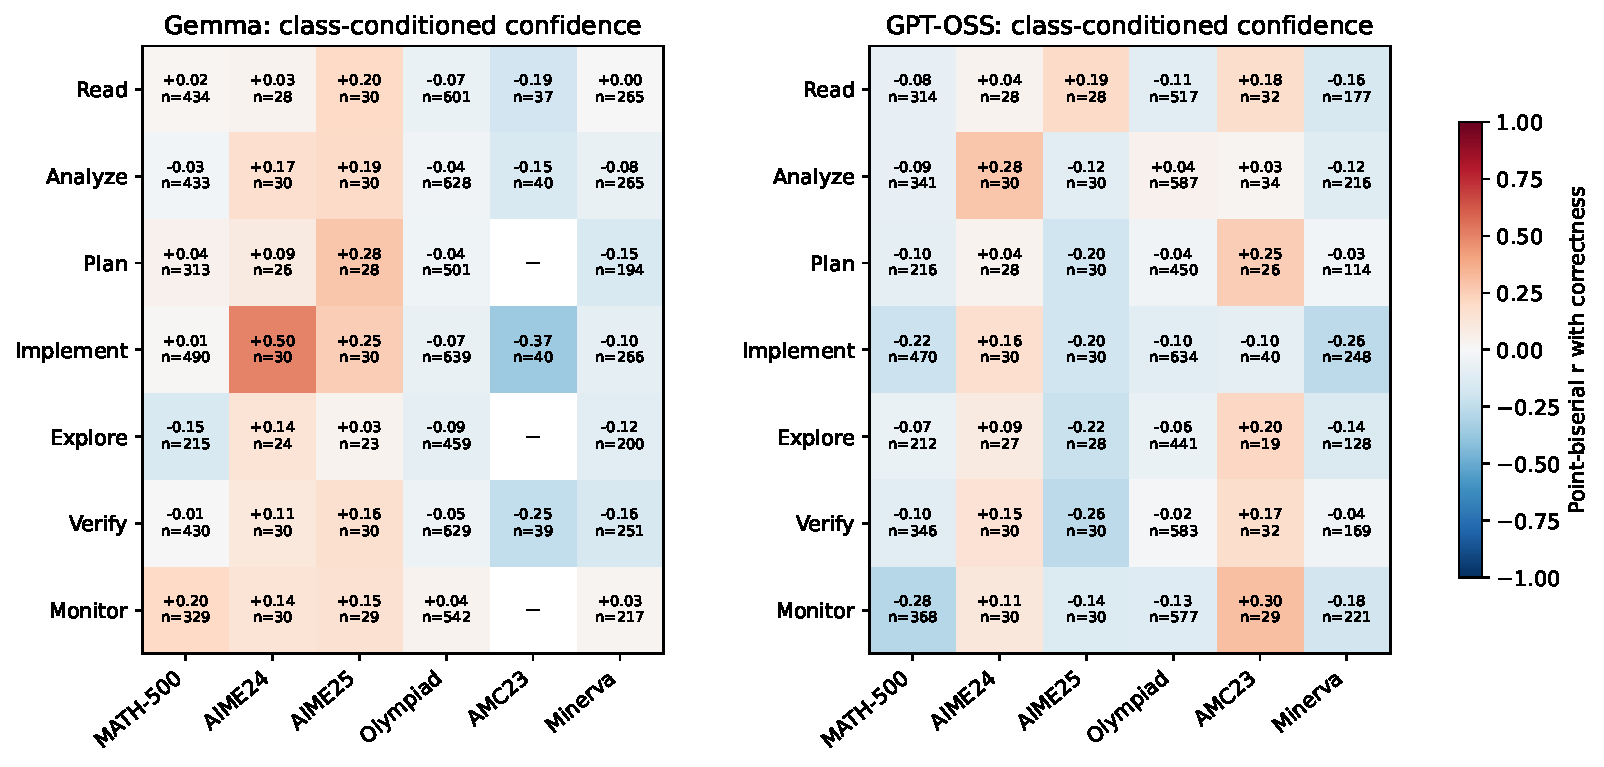
\includegraphics[width=\linewidth]{figures/stratified_class_confidence.pdf}
\caption{Class-conditioned router confidence versus whole-attempt correctness after stratified relabelling. Each cell reports the saved point-biserial coefficient and its finite-attempt count. Cohorts include only attempts with tokens assigned to that class; missing coefficients are undefined, not zero. Sparse AIME/AMC samples, near-ceiling outcomes, and model-specific problem selection limit comparisons. This descriptive screen does not adjust for length or difficulty or establish a causal class effect.}
\Description{Class-conditioned router confidence versus whole-attempt correctness after stratified relabelling. Each cell reports the saved point-biserial coefficient and its finite-attempt count. Cohorts include only attempts with tokens assigned to that class; missing coefficients are undefined, not zero. Sparse AIME/AMC samples, near-ceiling outcomes, and model-specific problem selection limit comparisons. This descriptive screen does not adjust for length or difficulty or establish a causal class effect.}
\end{figure}

The common annotation procedure improves benchmark coverage but does not match model cohorts. Full class/metric matrices are in the appended atlases. Qwen retains its earlier sampling and judge deployment, so the three-model class comparisons are not a controlled model comparison.
